\documentclass[11pt,a4paper]{article}
\usepackage[utf8]{inputenc}
\usepackage{amsmath}
\usepackage{pdflscape}
\usepackage{amsfonts}
\usepackage{float}
\usepackage{graphicx}
\usepackage{amssymb}
\usepackage{parskip}
\title{\vspace{-2.0cm} Assignment 1}
\author{Celina Ma, John Ngo, Omar Qureshi}
\begin{document}
\maketitle

\section*{Deliverable \#1}

Generally, the software development model is chosen in response to the circumstances of the software’s development. Our client is a real-world client – Professor Jason Donev, who is an individual and understandably has a busy schedule. He can meet up with us around once a week, but it would be difficult and unreasonable to remain in constant communication. There are difficulties for us as well as students going to classes on a set schedule, thus any method which requires constant client input and interaction on every aspect of development appears unsuitable. This difficulty eliminates the Scrum model, due to it being an agile model which requires such constant communication.

Next, we must consider our requirements, or lack there of. As we currently understand it, our client has a general trajectory as to what sort of software product he wants, but not the full specification of what exactly is desired down to the last detail. Furthermore, future improvement ideas have been discussed and thought of as early as the very beginning of the project, such as integrating a similar but not identical device – the Geiger counter. These facts strongly point away from incremental models, towards iterative models. 

Furthermore, we are all inexperienced in this project, not knowing the full details of what we might need to learn to complete this project, thus we cannot easily and evenly divide up the project – ruling out the concurrent model directly. The waterfall model requires a more intensive discussion with the client period before dropping off the radar and just building the software, where the first half might demand more attention than can be reasonably provided and the latter half squanders our ability to contact him for more questions, clarifications, and demonstrations of prototypes. As such, the Waterfall model is no fit either.

Phased release also suffers from the same intense requirements gathering phase needed in the beginning, and the rolling out of the releases do not actually factor in input from the client, again squandering a major advantage of being able to meet with and discuss the project with our client. As such, phased release is also not a reasonable model.

We are now left with the Spiral and Opportunistic models. Of these, the Opportunistic model doesn’t factor in client communication, and is not a clear and reliable software development plan for any external client or larger project. The scope of our project is not so small that the opportunistic model can work, since an app with multiple parts is much larger than projects suited for opportunistic, such as brief Computer Science class assignments or small segments of code. This leaves the Spiral model.

The spiral model’s quick cycles complete with risk assessment, planning and development stages appear to fit perfectly for this setup. In these brief meetings, we can gather requirements from our client and demonstrate the project as it currently stands; as it is an iterative model we can accommodate for changes in the project requirements and for future upgrades. As such, Spiral is a near perfect fit for our situation, and as such will be used.

\section*{Deliverable \#2}

\subsection*{2-1: Functional Requrements (FRs)}

\vskip 3mm

1. "The app must be able to receive data from the muon detector."

This app must be able to communicate with the external piece of hardware in order to meet the criteria given by the client. 

\vskip 6mm

2. "The app must be able to display a 'live' reading from the muon detector."

Along with receiving input from the detector, it then must be able to display the stream of values outputted by the detector onto the phone. 

\vskip 6mm

3. "The app must be able to average out the last 10 readings when pressing the 'get reading' button"

While a live reading is displayed, the 'get reading' button takes a snapshot of the readings average and displays a constant value underneath the live readings. 

\vskip 6mm
4. "The app must be able to record the averaged  'get readings' in a table." 

Upon pressing the 'get reading' button, the value is averaged and stored into a table that is accessible in another part/menu of the application.

\vskip 6mm
5. "The app and all of its relevant code must be open source to further future academic endeavours."

The client has specified that the code must be accessible to the public. This would progress the learning experiences of future students who want to extend on the work (ie make an iOS version).  


\subsection*{2-2: Non Functional Requirements (NFRs)}

1. "The app should present the readings with two significant digits."

This allows the user to experience a non cluttered UI, removing unnecessary information This NFR would fall under the usability. 

\vskip 6mm

2. "The app should record the readings by making a smooth visual animation."

A transition animation is often desired to express the information in a clearer way. This NFR would fall under the usability category. 

\vskip 6mm

3. "The app should record the readings within 0.5s after pressing the 'get reading' button."

This ensures the user doesn't have to wait an unusually long amount of time to get the reading. It also stops the user from getting frustrated and pressing the button again needlessly. This NFR would fall under the response time category. 
\vskip 6mm
4. "The app should emit a feedback sound when the user presses the ‘get reading button’" 

Giving the user direct confirmation of their action being applied is helpful and again stops user from pressing the button unnecessarily. This NFR would fall under the usability category.

\vskip 6mm
5. "The app should present a message if the muon detector is connected or not."

This makes sure that a precondition of using the app is met, which is having the miniUSB cable plugged into the phone and detector. This NFR would fall under the learnability/usability category. 


\newpage

\section*{Deliverable \#3}

\subsection*{3-1: Choosing User Stories/Map}

The reason why we chose user stories over use cases is...

\subsection*{3-2: User Stories}

The three core functional requirements that the user (in our case Professor Donev) needs to accomplish are as follows: connect muon detector to phone, view muon detector data and save data from muon detector to a log. As such, three corresponding story cards are created; 


\begin{figure}[h]
  \centering
  
      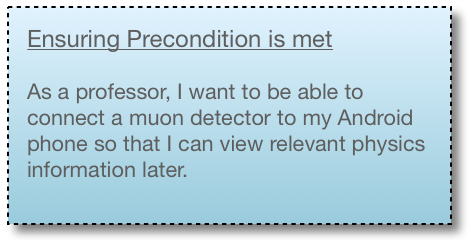
\includegraphics[width=0.7\textwidth]{storycard1.png}
      \caption{Individual story cards are first created to document core requirements, upon which further cards will be used to document how a user goes about accomplishing those tasks}
  
\end{figure}


\subsection*{3-3: Story Map}

With the use of the user story cards above, a collage/story map can be created that details further on how a user can interact with the app to accomplish their requirements. The story map can be viewed on the next landscape page. 

\newpage
\begin{landscape}
\begin{figure}[h]
  \centering
  
      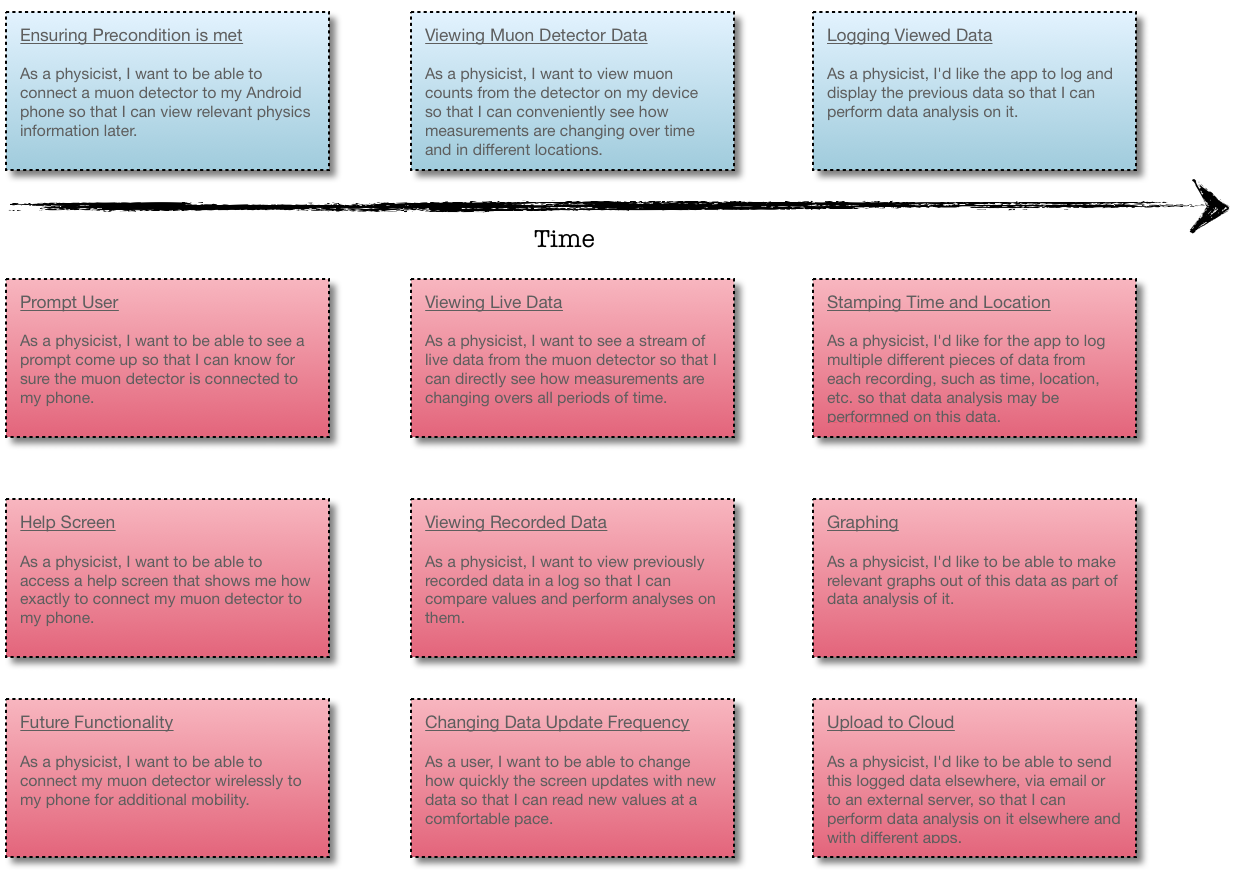
\includegraphics[width=1.6\textwidth]{storymap.png}
      \caption{A story map is used to organize requirements in order of priority and to illustrate how user interacts with app}
  
\end{figure}
\end{landscape}

\section*{Deliverable \#4}
\subsection*{4-1: Overview Sketches}
\bigskip
\begin{figure}[h]
  \centering
      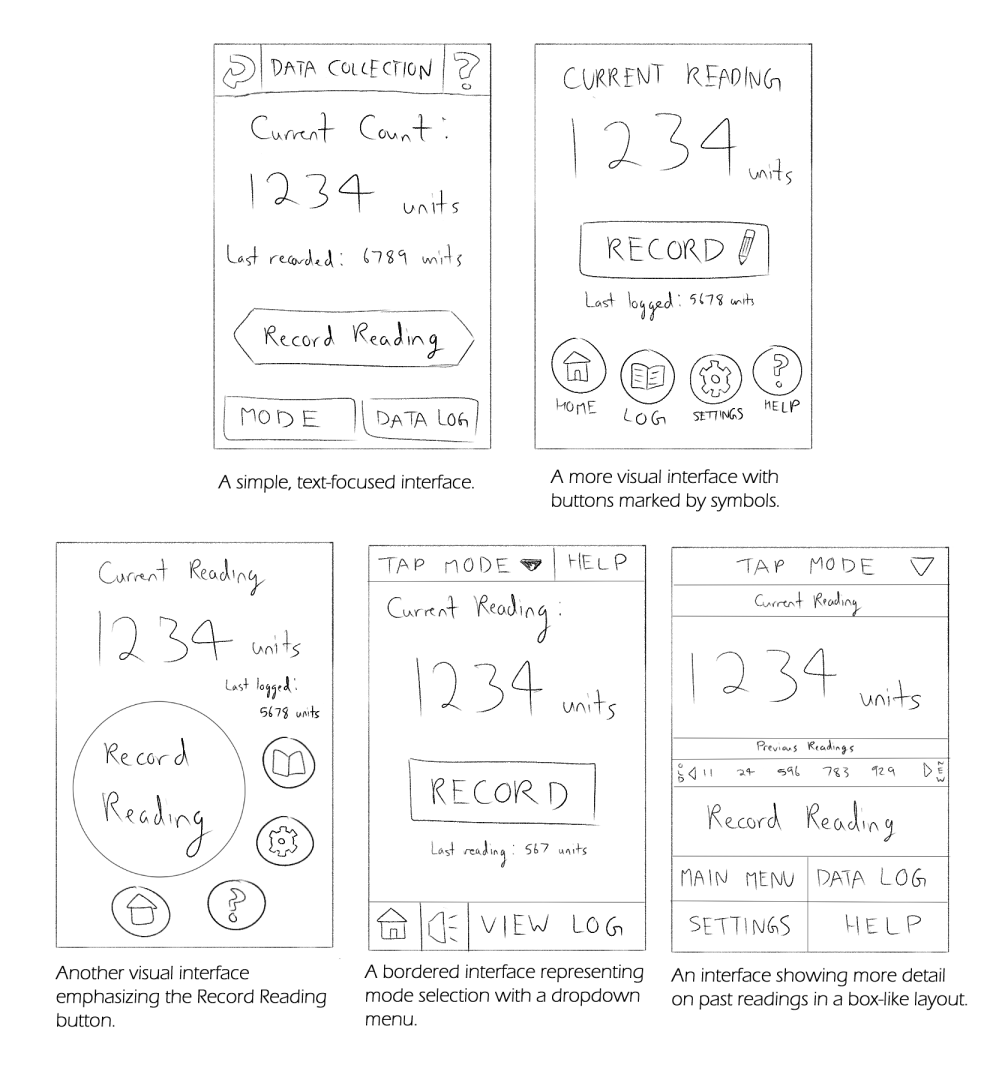
\includegraphics[width=1.1\textwidth]{overviewsketches.png}
  \caption{A variety of design approaches for the recording screen}
\end{figure}

\newpage
\subsection*{4-2: Elaborating Sketches}

\bigskip
\begin{figure}[h]
  \centering
      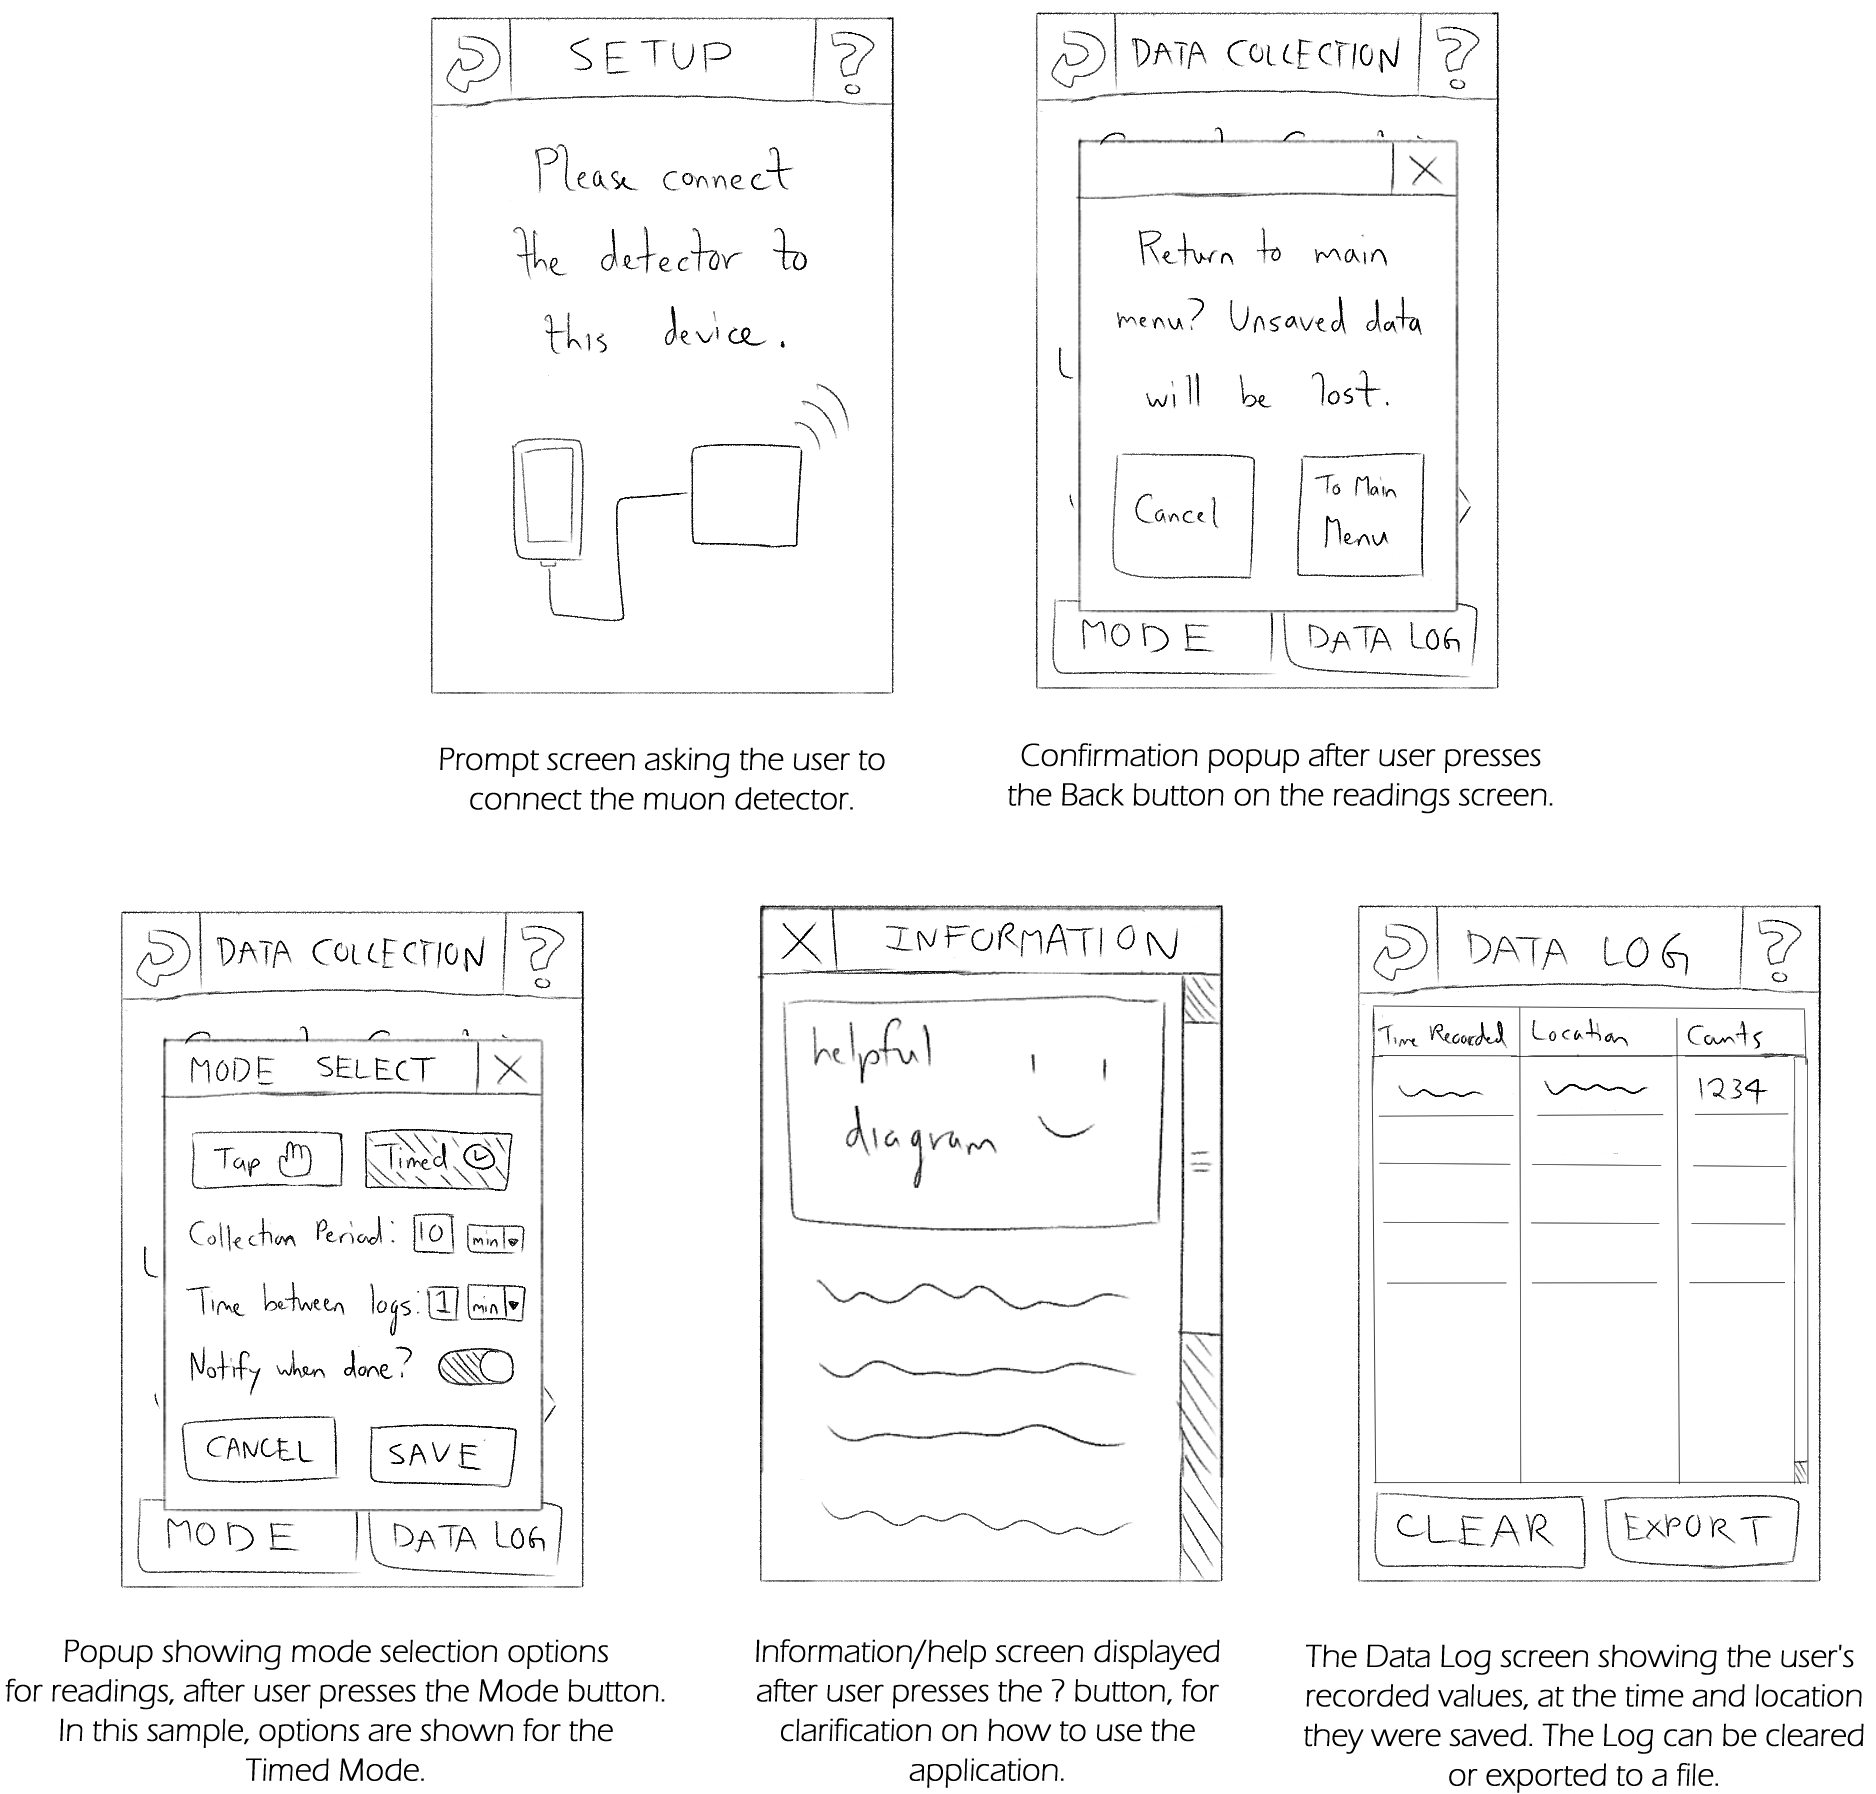
\includegraphics[width=1.2\textwidth]{elaboratingsketches.png}
  \caption{Extended sketches for other parts of the apps UI screens}
\end{figure}
\newpage
\subsection*{4-3: Storyboard Sketches}

\bigskip
\begin{figure}[h]
  \centering
      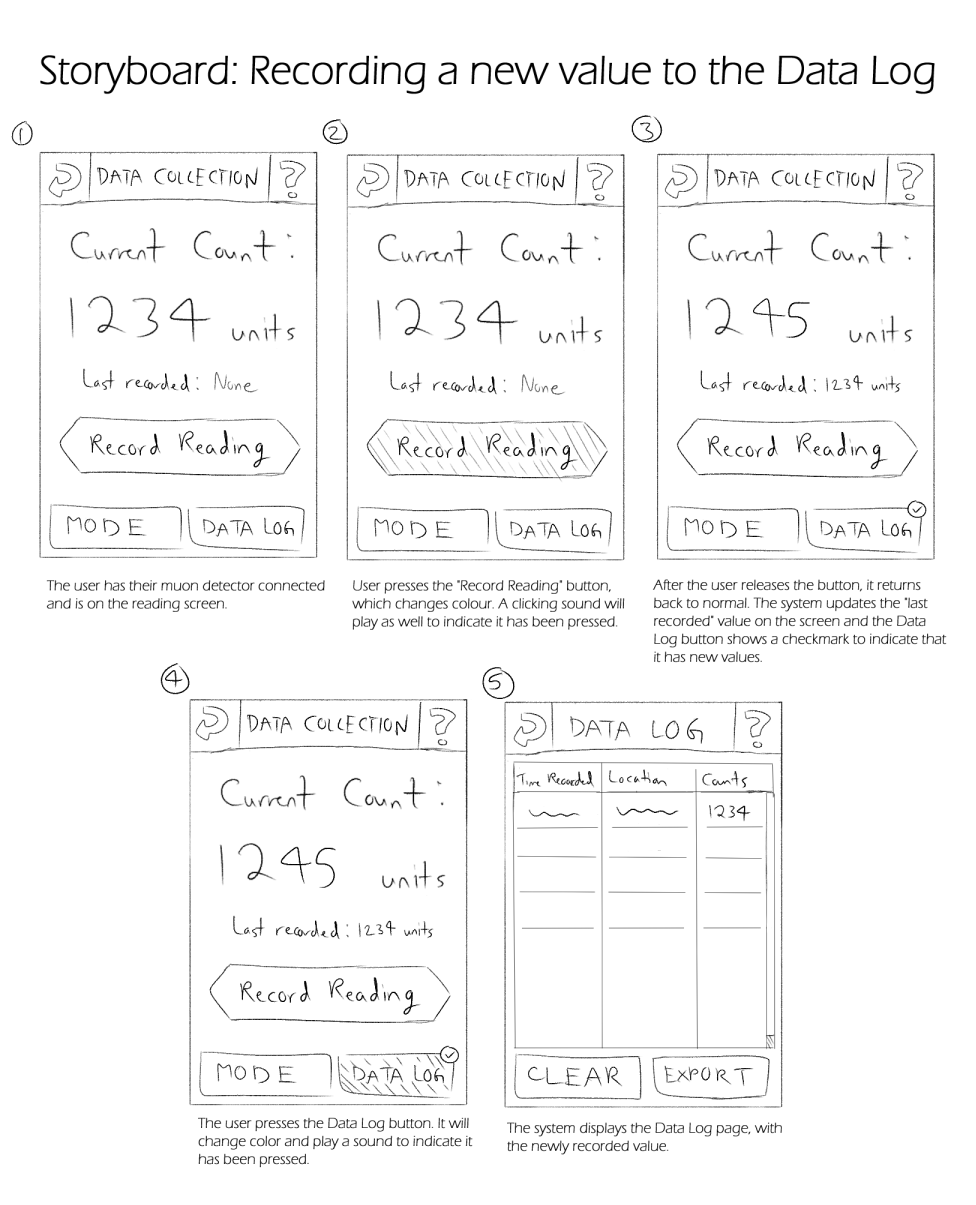
\includegraphics[width=0.98\textwidth]{storyboard.png}
  \caption{The recording screen responding to user input}
\end{figure}
\subsection*{4-3: Wizard of Oz Demo Video}
\subsection*{4-4: Requirements Change}
\section*{Deliverable \#5}

Our project first began with John consulting us about a program an external client, Dr. Donev,  might need. We agreed and this led to John emailing Dr. Donev  for confirming the project. The following emails show the first steps in the project; 
\bigskip
\begin{figure}[h]
  \centering
      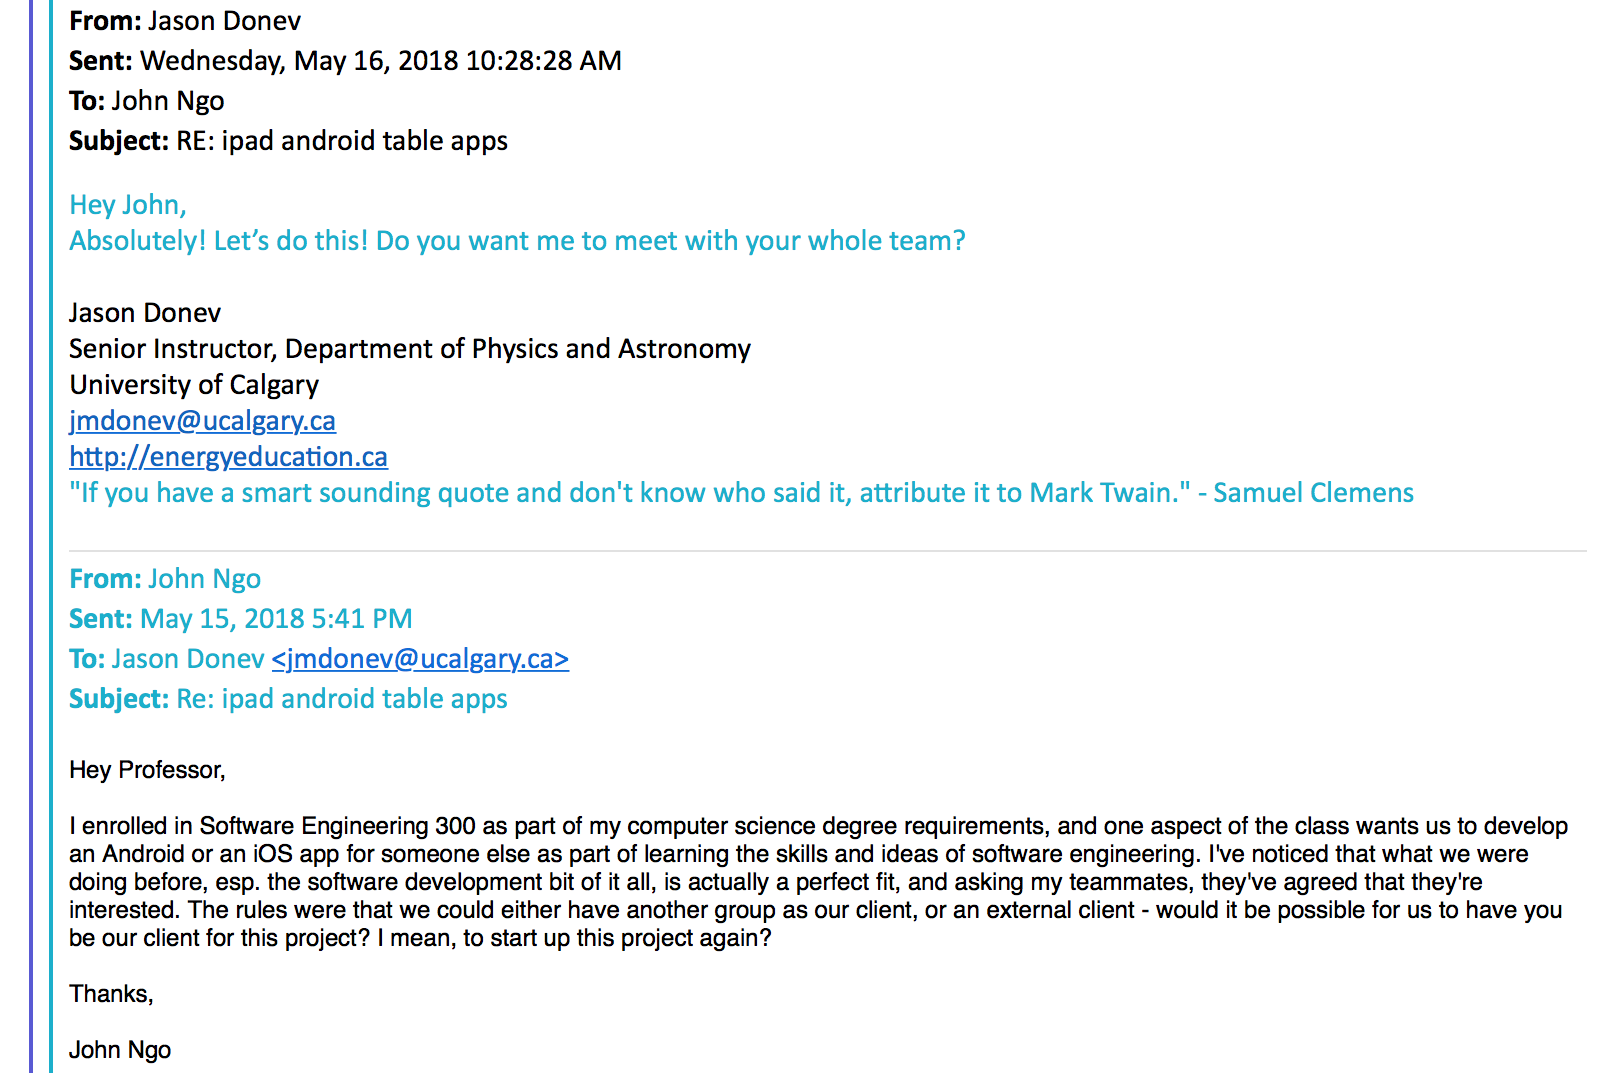
\includegraphics[width=0.8\textwidth]{1.png}
  \caption{Initial exchange of emails to get the project started}
\end{figure}

\newpage
Once the project was confirmed, Dr. Donev and John chatted briefly on the phone to go over some project specifications very briefly. John told us a little about the app requirements such as it needing to communicate with an external piece of hardware. After some discussions of our own, we then met with Dr. Donev as a group after confirming a time;


\bigskip
\begin{figure}[h]
  \centering
      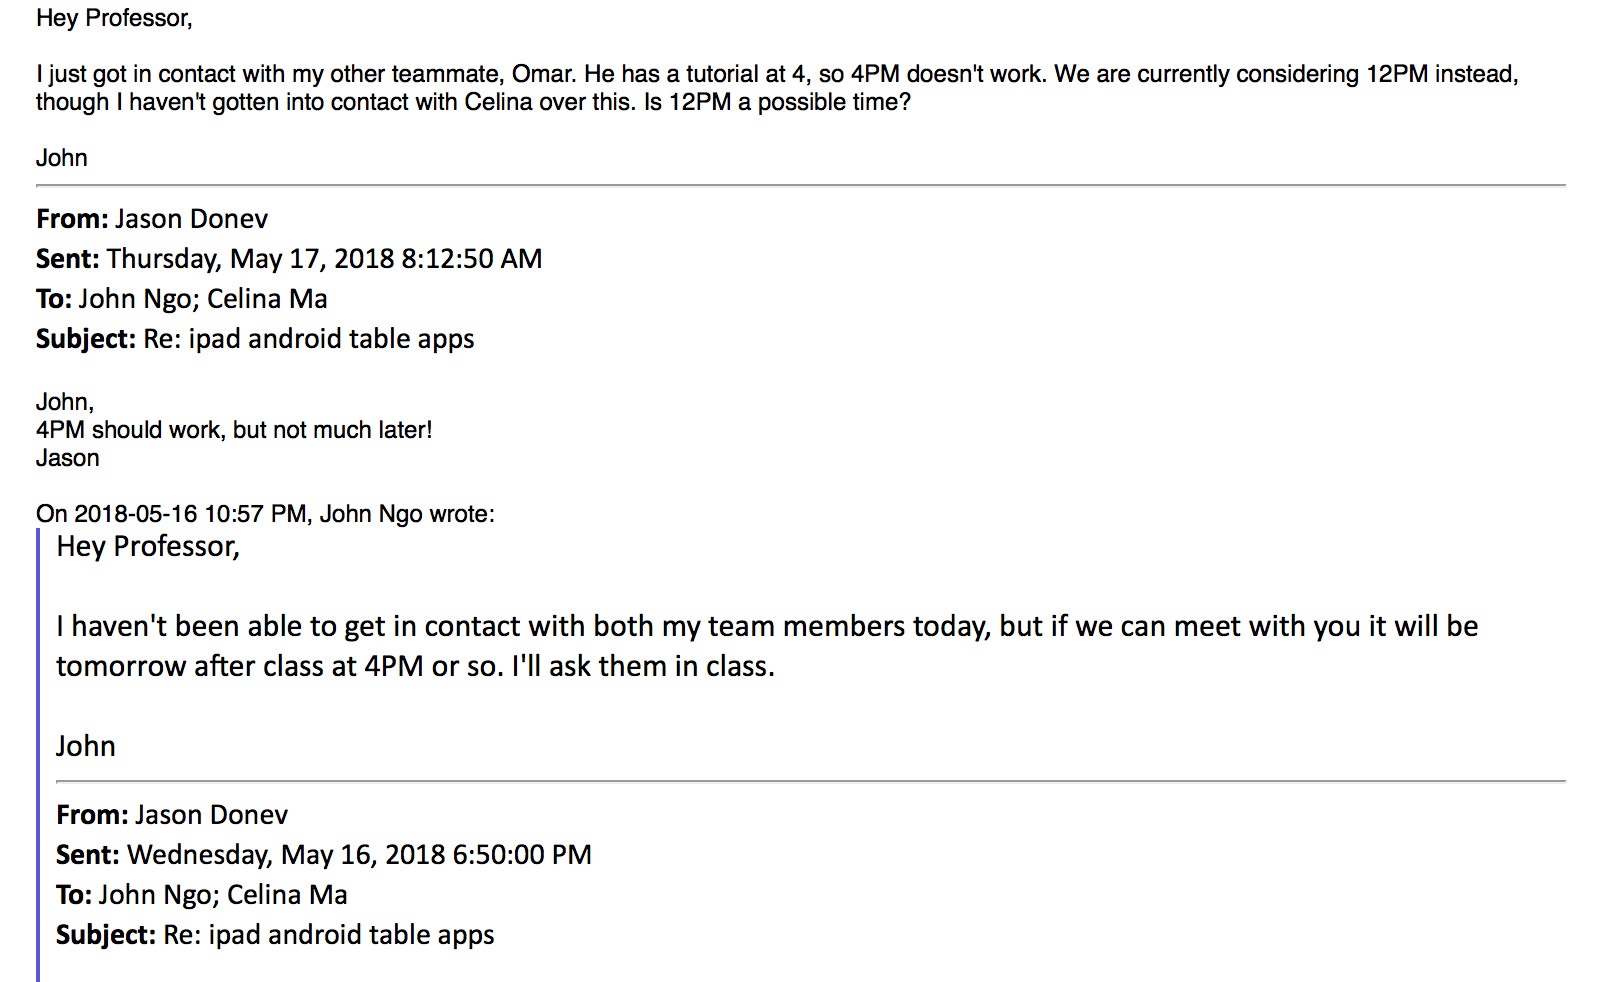
\includegraphics[width=0.8\textwidth]{3.png}

  \caption{Setting up a stand up meeting with Dr. Donev as a group}
\end{figure}


During this meeting we focused solely on requirements and what was the applications intended purpose. Some of the major requirements that were deduced were displaying a reading of the muons and being able to record that reading for data processing.

Approximately two weeks after the initial consult, we met with Dr. Donev again with a low fidelity prototype. This was the meeting where we recorded our Wizard of Oz style demo. 


\end{document}